\documentclass{amsart}
\usepackage[utf8]{inputenc}
\usepackage{amssymb}
\usepackage{amsthm}
\newtheorem{theorem}{Theorem}[section]
\usepackage{listings}
\usepackage{xcolor}
\usepackage{hyperref}
\usepackage{microtype}
\usepackage{tikz}
\usetikzlibrary{arrows.meta}

% -----------------------------------------------------------------------
% Macros for subject-matter identifiers (used in literate entries)
% -----------------------------------------------------------------------
\newcommand{\leanHarmonicInterval}{\textsf{HarmonicInterval}}
\newcommand{\leanIsTritone}{\textsf{IsTritone}}
\newcommand{\leanisSelfInverse}{\textsf{isSelfInverse}}
\newcommand{\leanisPerfect}{\textsf{isPerfect}}
\newcommand{\leanselfInverseSet}{\textsf{selfInverseSet}}
\newcommand{\leannonSIReachable}{\textsf{nonSIReachable}}
\newcommand{\leanmajorMinorIntervals}{\textsf{majorMinorIntervals}}
\newcommand{\leanstepMM}{\textsf{stepMM}}
\newcommand{\leanunison}{\textsf{unison}}

% -----------------------------------------------------------------------
% Lean listing style
% -----------------------------------------------------------------------
\lstdefinelanguage{Lean4}{
  % General structural keywords — 80% white
  keywords={abbrev,by,class,def,else,end,fun,if,in,inductive,instance,
            let,match,namespace,noncomputable,opaque,open,private,public,
            section,structure,then,true,variable,where,with},
  % Built-in tactics/strategies — 50% white
  keywords=[2]{apply,by_cases,calc,constructor,decide,exact,ext,fin_cases,
               have,haveI,intro,interval_cases,linear_combination,norm_num,
               obtain,omega,rcases,refine,rfl,ring,rintro,rw,rwa,simp,
               subst,unfold},
  % Declaration keywords — 20% white
  keywords=[3]{axiom,lemma,theorem},
  sensitive=true,
  morecomment=[l]{--},
  morestring=[b]",
}

\definecolor{leanKeyLight}{gray}{0.8}
\definecolor{leanKeyMid}{gray}{0.5}
\definecolor{leanKeyDark}{gray}{0.2}

\lstset{
  language=Lean4,
  basicstyle=\ttfamily\small,
  keywordstyle=\bfseries\color{leanKeyLight},
  keywordstyle=[2]\bfseries\color{leanKeyMid},
  keywordstyle=[3]\bfseries\color{leanKeyDark},
  commentstyle=\itshape\color{gray},
  columns=flexible,
  keepspaces=true,
  showstringspaces=false,
  breaklines=true,
  frame=none,
  numbers=left,
  numberstyle=\footnotesize,
  numbersep=8pt,
  stepnumber=2,
  extendedchars=true,
  inputencoding=utf8,
  literate=
    {HarmonicInterval}{\leanHarmonicInterval}{14}
    {IsTritone}{\leanIsTritone}{9}
    {isSelfInverse}{\leanisSelfInverse}{12}
    {isPerfect}{\leanisPerfect}{9}
    {selfInverseSet}{\leanselfInverseSet}{14}
    {nonSIReachable}{\leannonSIReachable}{14}
    {majorMinorIntervals}{\leanmajorMinorIntervals}{19}
    {stepMM}{\leanstepMM}{6}
    {unison}{\leanunison}{6}
    {ℕ}{$\mathbb{N}$}{1}
    {ℤ}{$\mathbb{Z}$}{1}
    {∀}{$\forall$}{1}
    {∃}{$\exists$}{1}
    {∧}{$\wedge$}{1}
    {∨}{$\vee$}{1}
    {¬}{$\neg$}{1}
    {→}{$\to$}{1}
    {↔}{$\leftrightarrow$}{1}
    {∈}{$\in$}{1}
    {∉}{$\notin$}{1}
    {∩}{$\cap$}{1}
    {∪}{$\cup$}{1}
    {≤}{$\leq$}{1}
    {≥}{$\geq$}{1}
    {≠}{$\neq$}{1}
    {⊂}{$\subset$}{1}
    {⊆}{$\subseteq$}{1}
    {⁻¹}{${}^{-1}$}{1}
    {⊢}{$\vdash$}{1}
    {·}{$\cdot$}{1}
    {λ}{$\lambda$}{1}
    {‹}{$\langle$}{1}
    {›}{$\rangle$}{1}
    {⟨}{$\langle$}{1}
    {⟩}{$\rangle$}{1}
    {∣}{$\mid$}{1}
    {▸}{$\triangleright$}{1}
    {←}{$\leftarrow$}{1}
    {=>}{$\implies$}{1}
}

% -----------------------------------------------------------------------
\title{12-Tone Equal Temperament: a Lean~4 Proof}
\author{Keith Braithwaite}
\date{\today}

\begin{document}
\maketitle

\begin{abstract}
We present a Lean~4 formalisation of the theorem that 12-tone equal
temperament (\textsc{12tet}) is the unique tuning system satisfying a
small set of musically-motivated axioms.  Intervals are modelled as
elements of $\mathbb{Z}/m\mathbb{Z}$.  The main theorem states $m = 12$;
a subsidiary theorem shows the major/minor interval class has exactly 8
members.
\end{abstract}

\tableofcontents

% -----------------------------------------------------------------------
\section{Introduction}
\label{sec:intro}
% -----------------------------------------------------------------------

In 12-tone equal temperament (\textsc{12tet}) the octave is divided into
12 equal semitones.  This paper asks: is there a small, musically
well-motivated set of axioms that \emph{forces} $m = 12$?  We answer yes,
by formalising the proof in Lean~4 with the Mathlib library.

\subsection*{Model}

Harmonic intervals are modelled as elements of $\mathbb{Z}/m\mathbb{Z}$
for an unknown $m$.  The four interval classes are:

\begin{description}
  \item[Unison] the identity element, $0$.
  \item[Tritone] the unique non-zero self-inverse element $t$ ($t + t = 0$).
  \item[Perfect] a primitive class constrained by axioms; exactly the
    pair $\{p, p^{-1}\}$.
  \item[Major/Minor] the least fixed point of a $\pm 1$ step operator
    starting from $\{p, p^{-1}\}$, stopping at $\{0, t\}$.
\end{description}

Inversion is additive negation: $i^{-1} = -i$.  This gives $i + i^{-1}
= 0$ by the ring axioms, corresponding to the musical fact that an
interval and its inverse span an octave.

\subsection*{The predicate \texorpdfstring{\textsf{isPerfect}}{isPerfect}}

The predicate \textsf{isPerfect} is declared \texttt{opaque} in Lean: it
has no explicit definition and can only be manipulated via the axioms.
This is essential.  Defining it as $i \neq 0 \wedge \neg\,\textsf{isSelfInverse}\,i$
would make every major/minor interval ``perfect'', collapsing the four
classes to two.

\lstinputlisting[
  firstline=49, lastline=49, firstnumber=49,
  caption={\texttt{Basic.lean}: the opaque perfect-interval predicate},
  label={lst:basic-perfect}
]{../Music/Basic.lean}

\subsection*{Module architecture}

Figure~\ref{fig:architecture} shows the eight \texttt{.lean} files and
their import dependencies.  Each rectangle lists the private declarations
inside; public declarations flow along the labelled arrows to the modules
that import them.

\begin{figure}[p]
\centering
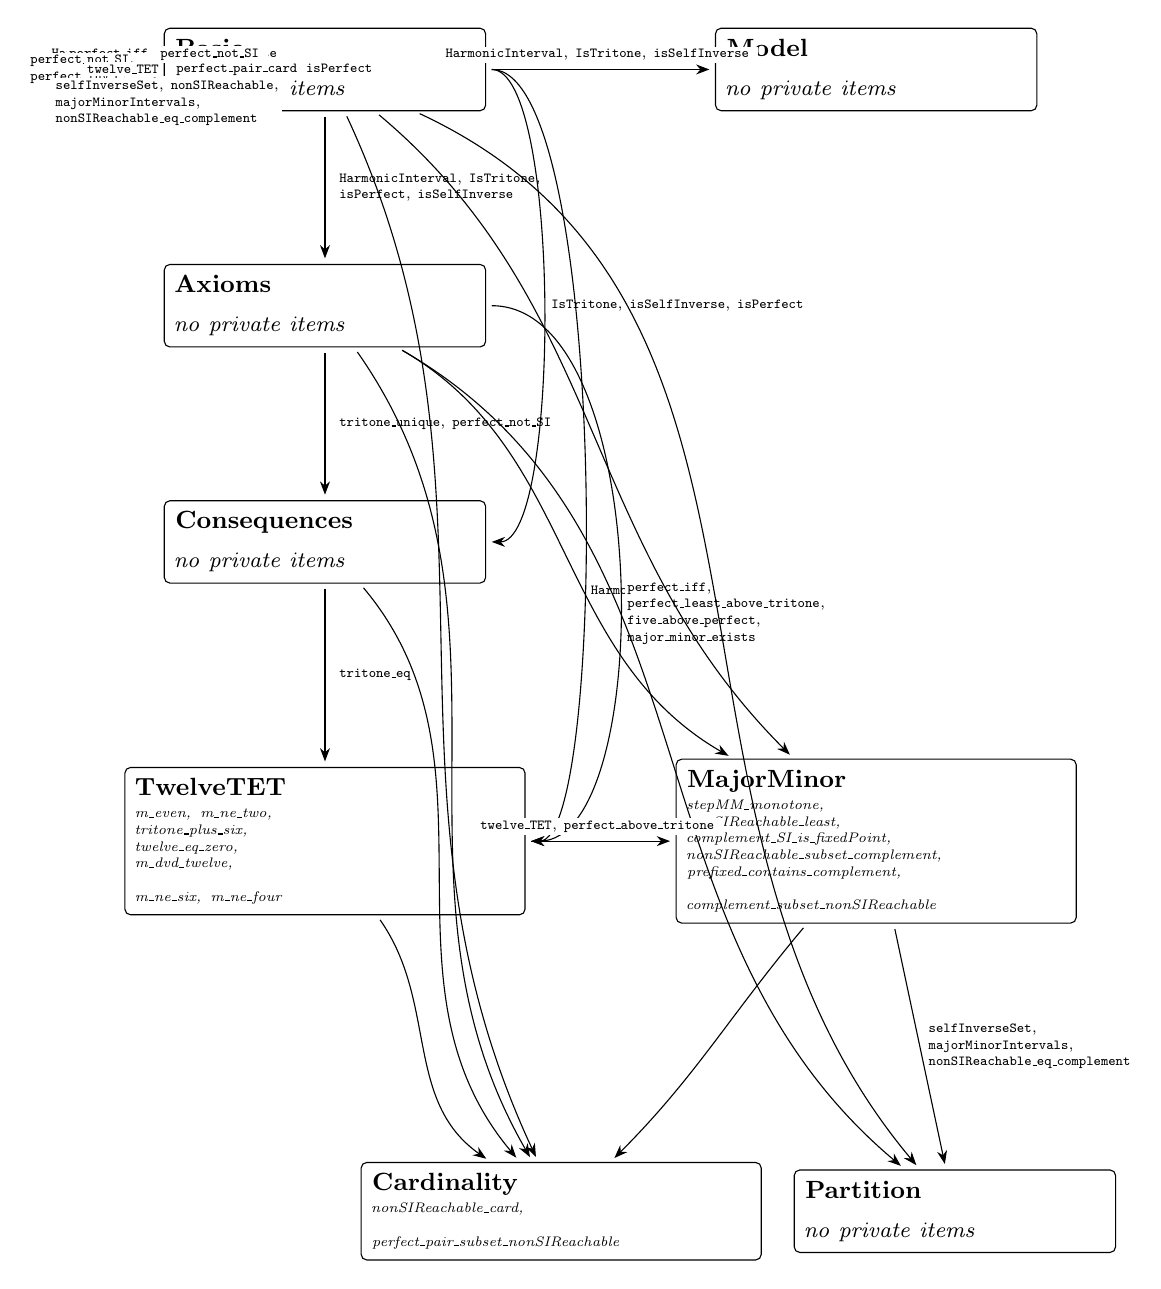
\begin{tikzpicture}[
  >=Stealth,
  mod/.style={draw, rectangle, rounded corners=2pt, text width=3.8cm,
              inner sep=4pt, align=left},
  modW/.style={draw, rectangle, rounded corners=2pt, text width=4.8cm,
               inner sep=4pt, align=left},
  imp/.style={->, thin, shorten >=2pt, shorten <=2pt},
  lbl/.style={font=\tiny, fill=white, inner sep=1pt, align=left}
]

%% ---- nodes ----
\node[mod] (basic) at (2, 0) {
  {\small\bfseries Basic}\\[2pt]
  \footnotesize\itshape no private items
};
\node[mod] (model) at (9, 0) {
  {\small\bfseries Model}\\[2pt]
  \footnotesize\itshape no private items
};
\node[mod] (axioms) at (2, -3) {
  {\small\bfseries Axioms}\\[2pt]
  \footnotesize\itshape no private items
};
\node[mod] (conseq) at (2, -6) {
  {\small\bfseries Consequences}\\[2pt]
  \footnotesize\itshape no private items
};
\node[modW] (twelve) at (2, -9.8) {
  {\small\bfseries TwelveTET}\\[2pt]
  \tiny\itshape
  m\_even, m\_ne\_two,\\
  tritone\_plus\_six,\\
  twelve\_eq\_zero,\\
  m\_dvd\_twelve,\\
  m\_ne\_six, m\_ne\_four
};
\node[modW] (mm) at (9, -9.8) {
  {\small\bfseries MajorMinor}\\[2pt]
  \tiny\itshape
  stepMM\_monotone,\\
  nonSIReachable\_least,\\
  complement\_SI\_is\_fixedPoint,\\
  nonSIReachable\_subset\_complement,\\
  prefixed\_contains\_complement,\\
  complement\_subset\_nonSIReachable
};
\node[modW] (card) at (5, -14.5) {
  {\small\bfseries Cardinality}\\[2pt]
  \tiny\itshape
  nonSIReachable\_card,\\
  perfect\_pair\_subset\_nonSIReachable
};
\node[mod] (part) at (10, -14.5) {
  {\small\bfseries Partition}\\[2pt]
  \footnotesize\itshape no private items
};

%% ---- main left-column chain ----

\draw[imp] (basic) -- (axioms)
  node[lbl, midway, right=4pt] {
    \texttt{HarmonicInterval}, \texttt{IsTritone},\\
    \texttt{isPerfect}, \texttt{isSelfInverse}
  };

\draw[imp] (axioms) -- (conseq)
  node[lbl, midway, right=4pt] {
    \texttt{tritone\_unique}, \texttt{perfect\_not\_SI}
  };

\draw[imp] (conseq) -- (twelve)
  node[lbl, midway, right=4pt] {\texttt{tritone\_eq}};

%% ---- skip arcs in left column, routed through east channel ----
%% Each arc bows right of the main chain boxes and re-enters from the east.

\draw[imp] (basic) .. controls (5.0, 0) and (5.0, -6) .. (conseq)
  node[lbl, pos=0.5, right=2pt] {
    \texttt{IsTritone}, \texttt{isSelfInverse}, \texttt{isPerfect}
  };

\draw[imp] (basic) .. controls (5.6, 0) and (5.6, -9.8) .. (twelve)
  node[lbl, pos=0.62, right=2pt] {
    \texttt{HarmonicInterval}, \texttt{isSelfInverse}
  };

\draw[imp] (axioms) .. controls (6.2, -3) and (6.2, -9.8) .. (twelve)
  node[lbl, pos=0.55, right=2pt] {
    \texttt{perfect\_iff},\\
    \texttt{perfect\_least\_above\_tritone},\\
    \texttt{five\_above\_perfect},\\
    \texttt{major\_minor\_exists}
  };

%% ---- Basic → Model (horizontal) ----

\draw[imp] (basic) -- (model)
  node[lbl, midway, above=2pt] {
    \texttt{HarmonicInterval}, \texttt{IsTritone}, \texttt{isSelfInverse}
  };

%% ---- cross-column arcs from left column ----

\draw[imp] (basic) to[out=-40, in=135] (mm)
  node[lbl, pos=0.38, above=2pt] {
    \texttt{HarmonicInterval}, \texttt{isSelfInverse}
  };

\draw[imp] (basic) to[out=-65, in=115] (card)
  node[lbl, pos=0.42, right=2pt] {
    \texttt{HarmonicInterval}, \texttt{isPerfect}
  };

\draw[imp] (basic) to[out=-25, in=130] (part)
  node[lbl, pos=0.3, above=2pt] {\texttt{HarmonicInterval}};

\draw[imp] (axioms) to[out=-30, in=150] (mm)
  node[lbl, pos=0.5, above=2pt] {
    \texttt{perfect\_iff}, \texttt{perfect\_not\_SI}
  };

\draw[imp] (axioms) to[out=-55, in=120] (card)
  node[lbl, pos=0.48, left=2pt] {
    \texttt{perfect\_not\_SI},\\
    \texttt{perfect\_inv\_closed}
  };

\draw[imp] (axioms) to[out=-30, in=140] (part)
  node[lbl, pos=0.32, below=2pt] {\texttt{perfect\_iff}};

\draw[imp] (conseq) to[out=-50, in=130] (card)
  node[lbl, pos=0.5, right=2pt] {\texttt{perfect\_pair\_card}};

%% ---- TwelveTET → MajorMinor (horizontal) and → Cardinality ----

\draw[imp] (twelve) -- (mm)
  node[lbl, midway, above=2pt] {
    \texttt{twelve\_TET}, \texttt{perfect\_above\_tritone}
  };

\draw[imp] (twelve) to[out=-55, in=145] (card)
  node[lbl, pos=0.55, left=2pt] {\texttt{twelve\_TET}};

%% ---- MajorMinor → Cardinality and Partition ----

\draw[imp] (mm) to[out=-130, in=45] (card)
  node[lbl, pos=0.5, below=3pt] {
    \texttt{selfInverseSet}, \texttt{nonSIReachable},\\
    \texttt{majorMinorIntervals},\\
    \texttt{nonSIReachable\_eq\_complement}
  };

\draw[imp] (mm) -- (part)
  node[lbl, midway, right=2pt] {
    \texttt{selfInverseSet},\\
    \texttt{majorMinorIntervals},\\
    \texttt{nonSIReachable\_eq\_complement}
  };

\end{tikzpicture}
\caption{Lean module architecture. Private declarations are listed in
  italics inside each rectangle. Each arrow is labelled with the public
  names from the source module that are used in the destination.}
\label{fig:architecture}
\end{figure}

% -----------------------------------------------------------------------
\section{Axioms}
\label{sec:axioms}
% -----------------------------------------------------------------------

We use eight axioms.  All are stated as Lean \texttt{axiom} declarations,
which are trusted without proof.

\subsection{A1 and A2: the tritone}

A non-zero self-inverse interval exists and is unique.  A1 forces $m$ to
be even; A2 rules out $m = 8$ (where both 2 and 6 are self-inverse).

\lstinputlisting[
  linerange={8-10,12-15}, firstnumber=8,
  caption={\texttt{Axioms.lean}: A1 and A2},
  label={lst:ax-tritone}
]{../Music/Axioms.lean}

\subsection{A3: a perfect interval exists}

\lstinputlisting[
  firstline=18, lastline=18, firstnumber=18,
  caption={\texttt{Axioms.lean}: A3},
  label={lst:ax-perfect-exists}
]{../Music/Axioms.lean}

\subsection{A4: perfect intervals are not self-inverse}

\texttt{perfect\_nonzero} is derived immediately from A4: since unison is
self-inverse, a perfect interval cannot be unison.

\lstinputlisting[
  linerange={21-23,25-27}, firstnumber=21,
  caption={\texttt{Axioms.lean}: A4 and derived \texttt{perfect\_nonzero}},
  label={lst:ax-a4}
]{../Music/Axioms.lean}

\subsection{A5: the perfect class is exactly \texorpdfstring{$\{p, p^{-1}\}$}{the pair}}

\texttt{perfect\_unique} and \texttt{perfect\_inv\_closed} are derived
directly from A5 by taking the two directions of the biconditional.

\lstinputlisting[
  firstline=30, lastline=40, firstnumber=30,
  caption={\texttt{Axioms.lean}: A5 and derived consequences},
  label={lst:ax-a5}
]{../Music/Axioms.lean}

\subsection{A6: minimality of the perfect interval above the tritone}

Rather than asserting $p = t + 1$ directly (which would introduce an
unexplained literal), A6 states that $p$ is the \emph{least}
non-self-inverse element of $\mathbb{Z}/m\mathbb{Z}$ whose value exceeds
that of $t$.  The equation $p = t + 1$ is then \emph{derived} in
Section~\ref{sec:derived}.

\lstinputlisting[
  firstline=43, lastline=47, firstnumber=43,
  caption={\texttt{Axioms.lean}: A6},
  label={lst:ax-a6}
]{../Music/Axioms.lean}

\subsection{A7: five semitones above the perfect interval reaches unison}

This is the acoustic constraint.  It encodes the approximation
$\log_2(3/2) \approx 7/12$: the perfect fifth is 7 semitones, so its
inverse (the perfect fourth) is 5 semitones, and $7 + 5 = 12 = 0$ in
$\mathbb{Z}/12\mathbb{Z}$.

\lstinputlisting[
  firstline=50, lastline=51, firstnumber=50,
  caption={\texttt{Axioms.lean}: A7},
  label={lst:ax-a7}
]{../Music/Axioms.lean}

\subsection{A8: a major/minor interval exists}

This rules out $m = 4$.  In $\mathbb{Z}/4\mathbb{Z}$, the four elements
are fully accounted for by unison, tritone, and the perfect pair; there
is no room for a fourth class.

\lstinputlisting[
  firstline=54, lastline=56, firstnumber=54,
  caption={\texttt{Axioms.lean}: A8},
  label={lst:ax-a8}
]{../Music/Axioms.lean}

% -----------------------------------------------------------------------
\section{Derived Facts}
\label{sec:derived}
% -----------------------------------------------------------------------

\subsection*{Shared consequences}

\texttt{tritone\_eq} uses A2 (tritone uniqueness) to pin the tritone to a
concrete value in any specific modulus, by supplying a witness and
checking it satisfies the two defining properties.  This eliminates
repeated boilerplate in later proofs.

\lstinputlisting[
  firstline=8, lastline=27, firstnumber=8,
  caption={\texttt{Consequences.lean}: shared derived lemmas},
  label={lst:consequences}
]{../Music/Consequences.lean}

\subsection*{$m$ is even}

The tritone has additive order 2 (A1); the order of any element divides
the group order $|\mathbb{Z}/m\mathbb{Z}| = m$; hence $2 \mid m$.

\lstinputlisting[
  firstline=57, lastline=68, firstnumber=57,
  caption={\texttt{TwelveTET.lean}: $m$ is even},
  label={lst:even}
]{../Music/TwelveTET.lean}

\subsection*{$m \neq 2$}

Every element of $\mathbb{Z}/2\mathbb{Z}$ is self-inverse, contradicting A4.

\lstinputlisting[
  firstline=71, lastline=75, firstnumber=71,
  caption={\texttt{TwelveTET.lean}: $m \neq 2$},
  label={lst:ne-two}
]{../Music/TwelveTET.lean}

\subsection*{$p = t + 1$, derived from A6}

Since $m$ is even and $m \neq 2$ we have $m \geq 4$, so $2 \neq 0$ in
$\mathbb{Z}/m\mathbb{Z}$.  Therefore $t+1$ is not self-inverse (its
double is $2 \neq 0$).  By A6, $\mathrm{val}(p) \leq \mathrm{val}(t+1)
= \mathrm{val}(t) + 1$.  Combined with $\mathrm{val}(t) < \mathrm{val}(p)$
from A6, this forces $p = t + 1$.

\lstinputlisting[
  firstline=78, lastline=113, firstnumber=78,
  caption={\texttt{TwelveTET.lean}: $p = t + 1$ derived from minimality},
  label={lst:above}
]{../Music/TwelveTET.lean}

\subsection*{$m \mid 12$}

From $p = t+1$ and A7: $t + 6 = (t+1)+5 = p + 5 = 0$.  Then
$12 = 2(t+6)-(t+t) = 0$ in $\mathbb{Z}/m\mathbb{Z}$, so $m \mid 12$.

\lstinputlisting[
  linerange={116-122,124-129,131-134}, firstnumber=116,
  caption={\texttt{TwelveTET.lean}: $m \mid 12$},
  label={lst:dvd12}
]{../Music/TwelveTET.lean}

\subsection*{$m \neq 6$ and $m \neq 4$}

In $\mathbb{Z}/6\mathbb{Z}$: $t = 3$, $p = 4$, $p + 5 = 9 \neq 0$,
contradicting A7.  In $\mathbb{Z}/4\mathbb{Z}$: $t = 2$, $p = 3$,
$p^{-1} = 1$; every element is in $\{0, t, p, p^{-1}\}$, contradicting A8.

\lstinputlisting[
  linerange={137-144,146-158}, firstnumber=137,
  caption={\texttt{TwelveTET.lean}: eliminating $m = 6$ and $m = 4$},
  label={lst:ne-four-six}
]{../Music/TwelveTET.lean}

\subsection*{The 12TET theorem: $m = 12$}

Since $m \mid 12$, $m$ is even, and $m \notin \{2, 4, 6\}$, the only
remaining possibilities are $m \in \{12\}$ (with $m = 1$ excluded by
\texttt{NeZero}).  The \texttt{interval\_cases} tactic dispatches the
finite case split.

\lstinputlisting[
  firstline=161, lastline=171, firstnumber=161,
  caption={\texttt{TwelveTET.lean}: $m = 12$},
  label={lst:twelve-tet}
]{../Music/TwelveTET.lean}

\subsection*{Major/minor intervals as a least fixed point}

The major/minor class is defined as the least fixed point of the step
operator
\[
  \mathrm{stepMM}(p,t,s)
    = \bigl(s
        \cup \{j+1 \mid j \in s \cup \{p,p^{-1}\}\}
        \cup \{j-1 \mid j \in s \cup \{p,p^{-1}\}\}
      \bigr) \setminus \{0,t\}.
\]
The lfp is the intersection of all prefixed points (sets $s$ with
$\mathrm{stepMM}(p,t,s) \subseteq s$).

\lstinputlisting[
  linerange={30-32,34-39,41-57,60-72,74-76}, firstnumber=30,
  caption={\texttt{MajorMinor.lean}: definitions of \textsf{selfInverseSet}, \textsf{stepMM}, \textsf{nonSIReachable}, \textsf{majorMinorIntervals}},
  label={lst:mm-defs}
]{../Music/MajorMinor.lean}

The lfp equals the complement of the self-inverse set.  The upper bound
is immediate from monotonicity; the lower bound is proved by a 10-step
walk in $\mathbb{Z}/12\mathbb{Z}$ starting from $p = 7$ and $p^{-1} = 5$.

\lstinputlisting[
  linerange={81-92,94-97}, firstnumber=81,
  caption={\texttt{MajorMinor.lean}: upper bound},
  label={lst:mm-upper}
]{../Music/MajorMinor.lean}

\lstinputlisting[
  linerange={123-190,193-201,204-210}, firstnumber=123,
  caption={\texttt{MajorMinor.lean}: lower bound (10-step walk) and equality},
  label={lst:mm-lower}
]{../Music/MajorMinor.lean}

\subsection*{Cardinality}

\begin{theorem}
The major/minor class has $m - 4$ elements; in \textsc{12tet}, exactly~8.
\end{theorem}

\lstinputlisting[
  linerange={15-39,41-52,54-57}, firstnumber=15,
  caption={\texttt{Cardinality.lean}},
  label={lst:card}
]{../Music/Cardinality.lean}

% -----------------------------------------------------------------------
\section{The Partition Theorem}
\label{sec:partition}
% -----------------------------------------------------------------------

\begin{theorem}
The four classes --- $\{0\}$, $\{t\}$, $\{p, p^{-1}\}$, and the
major/minor class --- partition $\mathbb{Z}/m\mathbb{Z}$.
\end{theorem}

\lstinputlisting[
  firstline=11, lastline=29, firstnumber=11,
  caption={\texttt{Partition.lean}},
  label={lst:partition}
]{../Music/Partition.lean}

% -----------------------------------------------------------------------
\section{Risks to Validity}
\label{sec:risks}
% -----------------------------------------------------------------------

\subsection*{Axiom consistency}

Since \textsf{isPerfect} is opaque, the axioms cannot be proved as theorems.
We address this by bundling the eight axiom conditions into a structure
\texttt{HarmonicModel}, parameterised over an explicit predicate \texttt{perf}
that stands in for \textsf{isPerfect}.  A term of this type for a specific
modulus is a consistency certificate.

\lstinputlisting[
  linerange={21-24,26,28,30,32,34,36-38,40,42-43,46-66}, firstnumber=21,
  caption={\texttt{Model.lean}: axiom bundle and consistency certificate},
  label={lst:model}
]{../Music/Model.lean}

The model is $\mathbb{Z}/12\mathbb{Z}$ with $t = 6$, $p = 7$, and
$\mathrm{perf}\,i \Leftrightarrow i = 7 \vee i = 5$.  All eight conditions
are discharged computationally by \texttt{decide} or \texttt{fin\_cases} followed
by \texttt{decide}.

\subsection*{The numeral 5 in A7}

Axiom A7 ($p + 5 = 0$) introduces the literal 5.  This is the irreducible
acoustic content of the proof: the perfect fifth is approximated by 7/12
of an octave, a fact about physics that cannot be derived from qualitative
musical structure alone.  Any reformulation of A7 that avoids the numeral
5 must implicitly encode the same information.

\subsection*{The minimality axiom A6}

The minimality formulation of A6 avoids the literal 1 of the original
$p = t + 1$, but the derived lemma \texttt{perfect\_above\_tritone}
still concludes $p = t + 1$.  The improvement is that the \emph{axiom}
is now qualitative; the numeral emerges from the proof rather than being
assumed.

\subsection*{The opaque predicate \textsf{isPerfect}}

Declaring \textsf{isPerfect} opaque is load-bearing: it prevents Lean from
unfolding a hypothetical explicit definition during proof search, which
could produce spurious proofs.  The trade-off is that \textsf{isPerfect}
cannot be computationally evaluated.

% -----------------------------------------------------------------------
\section{Further Work}
\label{sec:further}
% -----------------------------------------------------------------------

\begin{itemize}
  \item \textbf{Formalise a model.}  Construct $\mathbb{Z}/12\mathbb{Z}$
    explicitly with $t = 6$, $p = 7$, and verify all eight axioms, giving
    a consistency proof.

  \item \textbf{Eliminate A7.}  Replace $p + 5 = 0$ with an axiom
    expressing acoustic nearness (best rational approximation of
    $\log_2(3/2)$) and derive $p + 5 = 0$ as a theorem.  This requires
    bringing in real analysis or continued-fraction arithmetic.

  \item \textbf{Diatonic structure.}  Characterise the major scale as a
    specific 7-element subset of the major/minor class and derive its
    interval structure (tone--semitone pattern) from the axioms.

  \item \textbf{Voice-leading.}  Formalise the claim that the major/minor
    class is closed under minimal voice-leading displacement ($\pm 1$ step),
    connecting the lfp construction to the musical concept.
\end{itemize}

% -----------------------------------------------------------------------
\appendix
\section{Lean~4 Proof Tactics}
\label{app:tactics}
% -----------------------------------------------------------------------

The following tactics appear in the proof.  Each entry gives the tactic
name as it appears in the source, followed by a brief plain-English
description of what it does.

\begin{description}
  \item[\texttt{apply}]
    Unify the current goal with the conclusion of a given lemma or
    hypothesis, leaving the lemma's hypotheses as new sub-goals.

  \item[\texttt{by\_cases}]
    Split the proof into two branches by introducing a hypothesis \(h : P\)
    in one branch and \(h : \neg P\) in the other.

  \item[\texttt{by\_contra}]
    Replace the current goal \(P\) with the assumption \(\neg P\) and
    derive a contradiction.

  \item[\texttt{calc}]
    Chain a sequence of equalities or inequalities, where each step is
    justified by a tactic or term.

  \item[\texttt{constructor}]
    Split a conjunction or existential goal into its components, producing
    one sub-goal per component.

  \item[\texttt{decide}]
    Discharge a decidable proposition by computation (kernel-level
    evaluation).

  \item[\texttt{exact}]
    Close the current goal by providing a term whose type matches it
    exactly.

  \item[\texttt{ext}]
    Reduce an equality of functions, sets, or finsets to pointwise
    equality, introducing a universally quantified variable.

  \item[\texttt{fin\_cases}]
    Enumerate all cases for a variable ranging over a finite type, reducing
    the goal to one instance per element.

  \item[\texttt{have}]
    Introduce a local hypothesis by stating its type and providing a proof;
    the main goal is then proved with the new hypothesis in context.

  \item[\texttt{haveI}]
    Like \texttt{have}, but inserts the result as a local instance so that
    typeclass search can use it immediately.

  \item[\texttt{interval\_cases}]
    When a variable is constrained to a finite range of integers by
    hypotheses in the context, enumerate each integer in that range as a
    separate case.

  \item[\texttt{intro}]
    Move a universally quantified variable or an implication hypothesis
    from the goal into the local context.

  \item[\texttt{linear\_combination}]
    Close a goal that is a linear combination of hypotheses by supplying
    the coefficients; the remainder is discharged by \texttt{ring}.

  \item[\texttt{norm\_num}]
    Evaluate and close goals involving numerical expressions (arithmetic,
    divisibility, inequalities on literals).

  \item[\texttt{nth\_rw}]
    Like \texttt{rw}, but rewrites only the \(n\)-th occurrence of the
    pattern rather than all occurrences.

  \item[\texttt{obtain}]
    Destruct a hypothesis of product, existential, or disjunctive type,
    binding the components to named variables.

  \item[\texttt{omega}]
    Decide linear arithmetic goals over the integers or natural numbers.

  \item[\texttt{push Not}]
    Push negations inward through logical connectives and quantifiers,
    converting e.g.\ $\neg(\forall x, P)$ to $\exists x, \neg P$.

  \item[\texttt{rcases}]
    Recursively destruct a hypothesis using a pattern, binding sub-terms
    to named variables in one step.

  \item[\texttt{refine}]
    Like \texttt{exact}, but allows placeholders (\texttt{?\_}) that
    become new sub-goals, supporting partial term construction.

  \item[\texttt{rfl}]
    Close a goal of the form $a = a$ by reflexivity.

  \item[\texttt{ring}]
    Close a goal that is an identity in a commutative (semi)ring by
    normalisation.

  \item[\texttt{rintro}]
    Combine \texttt{intro} and \texttt{rcases}: introduce a hypothesis and
    immediately destruct it using a pattern.

  \item[\texttt{rw}]
    Rewrite the goal (or a hypothesis) by substituting equals for equals,
    using an equation or iff.

  \item[\texttt{rwa}]
    Like \texttt{rw}, but closes the goal with \texttt{assumption} after
    the rewrite.

  \item[\texttt{simp}]
    Simplify the goal (or a hypothesis) by repeatedly applying a
    configurable set of rewrite lemmas and decision procedures.

  \item[\texttt{simp\_all}]
    Apply \texttt{simp} to the goal and all hypotheses simultaneously,
    using each simplified hypothesis to further simplify the others.

  \item[\texttt{subst}]
    Given a hypothesis $x = e$ (or $e = x$) where $x$ is a local
    variable, substitute $e$ for $x$ everywhere and remove the variable.

  \item[\texttt{unfold}]
    Unfold a definition by name in the goal, replacing the defined
    identifier with its body.
\end{description}

\end{document}
